% .:: Laden der LaTeX4EI Formelsammlungsvorlage
\documentclass[fs, footer]{latex4ei}
\usepackage[european]{circuitikz}

\usepackage{multirow}
\usepackage{latexnew}


% Dokumentbeginn
% =======================================================================
\begin{document}


% Aufteilung in Spalten
\vspace{-4mm}
\begin{multicols*}{4}
    \fstitle{Systemtheorie}

    \section{Reaktive Elemente}

    \subsection{Die vier zentralen Größen $u,i,q,\Phi$}
    % ----------------------------------------------------------------------
    ... beschreiben die Wirkungsweise von elektronischen Bauelementen.\\ \\
    \textbf{Spannung \textit{u}}: Potentialdifferenz. Hohes zu niedrigem Potential\\
    \textbf{Strom \textit{i}}: Bewegte Ladung. Bewegungsrichtung positiver Ladung\\
    \textbf{Ladung \textit{q}}: Grundeigenschaft von Materie.\\
    \textbf{Magnetischer Fluss \textit{$\Phi$}}: Grundeigenschaft von elektr. magn. Feldern\\
    \subsubsection{Allgemeine Zusammenhänge $u,i,q,\Phi$}
    Ladung und Strom beschreiben den Zustand der Materie.\\
    Spannung und magn. Fluss beschreiben den Zustand des elekt. magn. Feldes.\\
    Kondensator ist u-gesteuert (q-gesteuert), falls für ein u (q) nur ein q (u)  existiert. \\
    Induktivität ist i-gesteuert ($\phi$-gesteuert), falls für ein i ($\phi$) nur ein $\phi$ (i) existiert. \\
    \begin{tabular}{l|l}
        $i(t) = \dot q(t)$                                      & $[i]=A$        \\
        $q(t) = q(t_0) + \int_{t_0}^t i(\tau) \mathrm d\tau$    & $[q]=As=C$     \\ \hline
        $u(t) = \dot \Phi(t)$                                   & $[u]=V$        \\
        $\Phi = \Phi(t_0) + \int_{t_0}^t u(\tau) \mathrm d\tau$ & $[\Phi]=Vs=Wb$ \\
    \end{tabular}

    \subsubsection{Arten von Bauelementen}
    \begin{tabular}{l|l|l|l}
        Art           & Symbol                                                  & Beschr.       & linear                      \\ \hline
        Resistivität  & 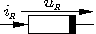
\includegraphics[height=0.4cm]{./img/Resistivitat.pdf}  & $f_R(u,i)$    & $u = U_0 + R \cdot i$       \\
        Kapazität     & 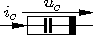
\includegraphics[height=0.4cm]{./img/Kapazivitat.pdf}   & $f_C(u,q)$    & $q = Q_0 + C \cdot u$       \\
        Induktivität  & 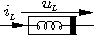
\includegraphics[height=0.4cm]{./img/Induktivitat.pdf}  & $f_L(i,\Phi)$ & $\Phi = \Phi_0 + L \cdot i$ \\
        Memristivität & 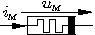
\includegraphics[height=0.4cm]{./img/Memristivitat.pdf} & $f_M(q,\Phi)$ & $\Phi = \Phi_0 + M \cdot q$ \\
    \end{tabular}
    \subsubsection{Zusammenhang der Bauelemente}
    \begin{center}
        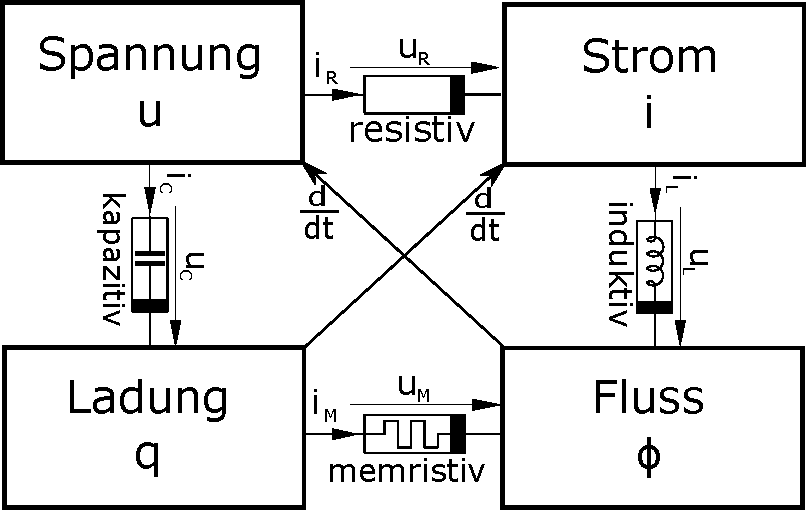
\includegraphics[scale=0.3]{./img/reactance_overview.pdf}
    \end{center}
    \subsubsection{Eigenschaften von Reaktanzen}
    \textbf{Linearität}: siehe Eintore\\
    \textbf{Differentialgleichung}: $i(t) = C \frac{\mathrm du(t)}{\mathrm dt}, u(t) = L \frac{\mathrm di(t)}{\mathrm dt}$\\
    \textbf{Gedächtnis}: Verhalten durch vorhergehende Klemmengrößen bestimmt.\\
    \textbf{Stetigkeit}: $u_C(t)$, $i_L(t)$ stetig in $(t_a, t_b)$, wenn Torgrößen endlich\\
    \textbf{Verlustfreiheit}: $W_C(t_1, t_2) = \int_{t_1}^{t_2}\! u(t)i(t)\,\mathrm dt = \int_{q_1}^{q_2}\! \mathrm{X}(q)\,\mathrm{d}t$ (Arbeit)\\
    Falls linear: $W = \frac{Cu^2}{2} = \frac{Li^2}{2}$\\
    Periodisch: $u(t+T) = u(t)$, $q(t+T) = q(t)$\\
    Graphisch: Falls keine geschlossenen Schleifen in q/u, $\Phi$/i-Diagramm existiert (Hystenesefrei)\\
    \textbf{Energie (nicht linearer Fall)}:\\
    - Kapazitiv: $W_C(t_1, t_2) = \int_{t_1}^{t_2} \! u(t)i(t)\, \mathrm dt = \int_{q_1}^{q_2} \! u(q)\, \mathrm dq$\\
    - Induktiv: $W_C(t_1, t_2) = \int_{t_1}^{t_2} \! u(t)i(t)\, \mathrm dt = \int_{\Phi_1}^{\Phi_2} \! i(\Phi)\, \mathrm d\Phi$\\
    \textbf{Energie (linearer Fall)}:\\
    - Kapazitiv: $W_C = \frac{C}{2}u^2 = \frac{1}{2C}q^2$\\
    - Induktiv: $W_L = \frac{L}{2}i^2 = \frac{1}{2L} \Phi^2$\\
    Graphisch: Fläche zwischen der Kennlinie und der q-/$\Phi$-Achse\\
    \textbf{Relaxationspunkte (=Ruhepunkte)}: Betriebspunkte, in dem die in einer Reaktanz gespeicherte Energie minimal ist. Kandidaten sind: Extremwerte, Wendepunkte, Knicke, Schnittpunkte mit q-/$\Phi$-Achse\\
    \subsubsection{Verschaltung von Reaktanzen}
    - Parallelschaltung: $C_p = C_1 + C_2$, $L_p = L_1 || L_2 = \frac{L_1L_2}{L_1+L_2}$\\
    - Serienschaltung: $C_p = C_1 || C_2 = \frac{C_1C_2}{C_1+C_2}$, $L_p = L_1 + L_2$\\


    Merke: Am Kondensa\textsl{tor}, eilt der Strom \textsl{vor}, bei Induktivi\textsl{täten}, wird er sich ver\textsl{späten}\\
    Merke: Ist das Mädchen brav, bleibt der Bauch konkav, hat das Mädchen Sex, wird der Bauch konvex.\\

    \subsubsection{Dualität}
    $u\rightarrow R_d\cdot i^d$, $i\rightarrow \frac{1}{R_d}u^d$\\
    $\Phi\rightarrow R_d\cdot q^d$, $q\rightarrow \frac{1}{r_d}\cdot\Phi^d$

    %TODO Markt & Population (Zitat Joham) S.19f.

    \section{Systeme ersten Grades}
    \sectionbox{
    \textbf{I. Resistives ESB bestimmen}\\
    \tablebox{
        \begin{tabular*}{\columnwidth}{@{\extracolsep\fill}l|ll@{}} \trule
            & Kapazität & Induktivität \\ \mrule
            ESB-Typ & Helmholtz-Thévinin & Mayer-Norton\\
            &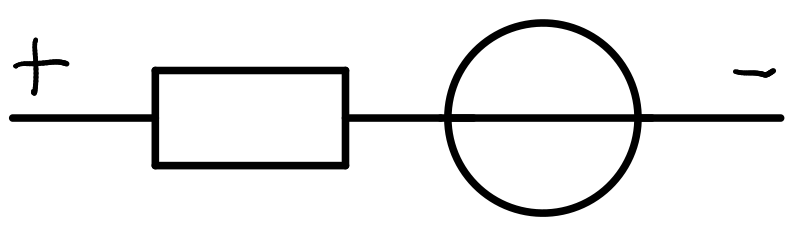
\includegraphics[width=.3\linewidth]{img/helmholtz-thevenin}&
            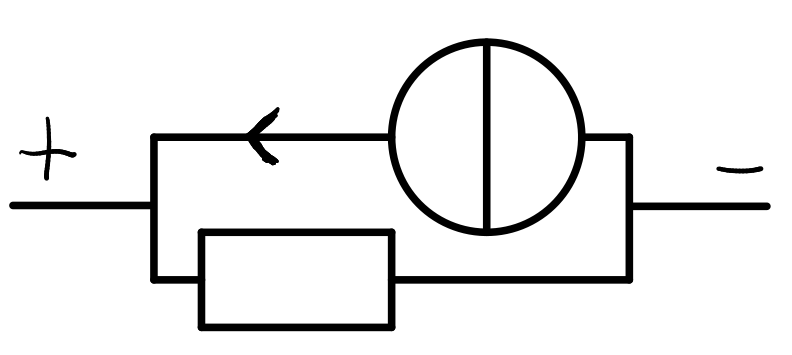
\includegraphics[width=.3\linewidth]{img/mayer-norton}\\
            Zustandsgröße & $x(t) = u_C(t)$ & $x(t) = i_L(t)$\\
            Zeitkonstante & $\tau = RC$ & $\tau = GL$\\
            \brule
        \end{tabular*}
    }

    \textbf{II. Aufstellen DGL} (kanonische Form)\\
    $\dot x(t) = - \fr{1}{\tau}x(t) + \fr{1}{\tau}v$ mit der Erregung $v$\\
    \textbf{III. Lösen der DGL}\\
    Konstante Erregung:  $x(t) = x_\infty + (x_0 - x_\infty )\e^{-\frac{t-t_0}{\tau}}$ \\
    Allgemeine Erregung: $x(t) = \underbrace{x_0\e^{\frac{t_0-t}{\tau}}}_{\text{zero-input-response}}+\underbrace{\int_{t_0}^t{\frac{1}{\tau}v(t')\e^{\frac{t'_0-t'}{\tau}}}}_{\text{zero-state-response}}$ \\
    mit $u_{C,\infty}=U_0$ bzw. $i_{L,\infty}=I_0$\\
    \textbf{IV. Dynamischer Pfad}\\
    \tablebox{
        \begin{tabular*}{\columnwidth}{@{\extracolsep\fill}ll@{}} \trule
            Kapazität & Induktivität\\ \mrule
            $i < 0$: $u$ wird größer & $u < 0$: $i$ wird größer\\
            $i > 0$: $u$ wird kleiner & $u > 0$: $i$ wird kleiner\\
            $i = 0$: GGP & $u = 0$: GGP\\
            \brule
        \end{tabular*}
    }
    \textbf{Toter Punkt:} kein GGP, aber Pfad kann nicht fortgesetzt werden \ra Sprung der nicht stetigen Größe ($i_C$ oder $u_L$)\\
    \textbf{Gleichgewichtspunkt (GGP):}\\
    \begin{tabular*}{\columnwidth}{@{\extracolsep\fill}ll@{}}
        Kapazität & Induktivität\\ \mrule
        $\dd{t}u_F = 0 \ra i_F = 0$ & $\dd{t}i_F = 0 \ra u_F = 0$\\
        \mrule
    \end{tabular*}
    \begin{itemize}
        \item[a)] stabil, falls der Pfad nicht aus diesem Punkt herausläuft
        \item[b)] instabil, falls der Pfad aus dem Punkt herausläuft
        \item[c)] virtuell, falls der Pfad in einen toten Punkt auf dem verlängertem Pfad auf der Achse läuft
    \end{itemize}
    }

    \subsection{Stabile Schaltung ($\tau > 0$)}
    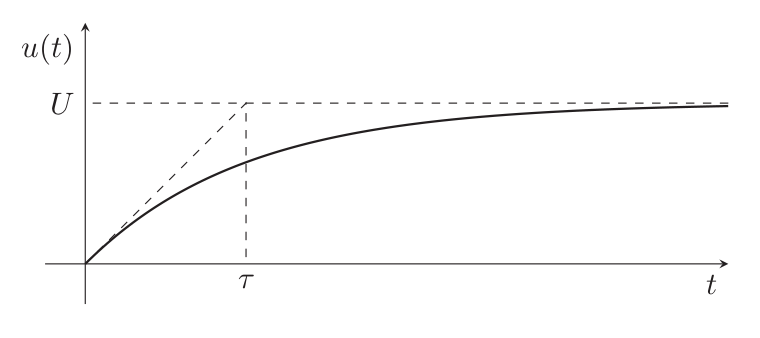
\includegraphics[width=.8\linewidth]{img/graph-stabil}
    \subsection{Instabile Schaltung ($\tau < 0$)}
    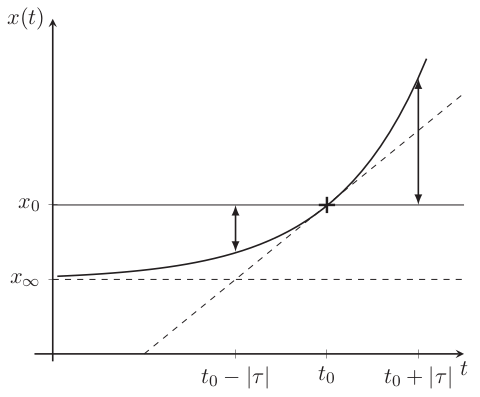
\includegraphics[width=.8\linewidth]{img/graph-instabil}
    \subsection{Dynamischer Pfad}
    %TODO Dynamischer Pfad S.24
    \subsection{Sprung- und Impulsantwort}\label{sec:Sprung- und Impulsantwort}
    \subsubsection{Sprungantwort}
    Sprungfunktion: $\sigma(t) = \begin{cases}1 & \text{für } t > 0 \\ 0 & \text{für } t < 0\end{cases}$\\
    Sprungantwort: $x_\sigma(t) = (1 - \exp{(-\fr{1}{\tau})})\sigma(t)$
    \subsubsection{Impulsantwort}
    rechteckförmiger Signalverlauf der Erregung\\
    Einheitsimpuls: $\delta(t) = \begin{cases}0 & \text{für } t \neq 0 \\ \infty & \text{für } t = 0$ und $\int_{-\epsilon_1}^{\epsilon_2}\delta(t)\diff t = 1 \quad \forall \epsilon_1, \epsilon_2 > 0\end{cases}$\\
    Impulsantwort: $h(t) = \fr{1}{\tau}\exp{(-\fr{1}{\tau})}\sigma(t) = \dd t \sigma$
    \subsection{Sprungphänomene}
    Tritt auf, falls Pfad in einen toten Punkt läuft.\\
    Führt zu einer sprungartigen Fortsetzung des dynamischen Pfades auf einem anderen Kennlinienast (Stetigkeitsregel beachten).\\
    Beispiele: Relaxationsoszilator, astabiler Multivibrator

    %TODO Sprungphänomene S.26

    %TODO Solow-Swan-Modell S.35
    \section{Systeme zweiten Grades}
    \subsection{Differentialgleichungssystem aufstellen}
    \textbf{I. Schaltung umzeichnen}\\
    Zeichne die Schaltung so um, dass beide Reaktanzen an den äußeren Seiten sind.\\
    \textbf{II. Matrix aufstellen}
    (Quellen vernachlässigen)
    \begin{itemize}
        \item[a)] zwei Kondensatoren: Leitwertsmatrix $\ma G$
        \item[b)] zwei Spulen: Widerstandsmatrix $\ma R$
        \item[c)] Kondensator (Tor 1) und Spule (Tor 2): Inverse Hybridmatrix $\ma{H'}$
        \item[d)] Spule (Tor 1) und Kondensator (Tor 2): Hybridmatrix $\ma{H}$
    \end{itemize}

    \textbf{III. Quellenvektor aufstellen}

    \textbf{IV. Differentialgleichungssystem aufstellen}
    \subsection{Phasenportraits}
    \subsubsection{Zeichnen des Phasenportraits}
    \textbf{I. Bestimmung der Eigenwerte $\lambda_i$ und Eigenvektoren $q_i$}\\
    $\lambda_{1,2} = \frac{tr(\ma A)}{2} \pm \sqrt{\frac{tr(\ma A)^2}{4}-det(\ma A)}$\\
    $a_{12} \neq 0 \Rightarrow \v q_i = \mat{-a_{12}\\a_{11}-\lambda_i}$\quad $a_{21} \neq 0 \Rightarrow \v q_i = \mat{a_{22}-\lambda_i\\-a_{21}}$\quad$a_{12} = a_{21} = 0 \Rightarrow \v q_1 = \mat{1\\0}, \v q_2 = \mat{0\\1}$\\
    Falls Eigenvektoren komplex: $\v q_r = Re\{q_1\}$\qquad$\v q_i = Im\{q_1\}$\\
    \textbf{II. Bestimmung des Fixpunktes}\\
    $\ma A\v x_\infty + \ma B\v v = 0 \Rightarrow \v x_\infty = -\ma A^{-1} \ma B\v v$\\
    %TODO Wtf
    \textbf{III. Art des Phasenportraits}\\
    \textbf{Strudelpunkt}\\
    $\lambda_{1/2} = \alpha \pm \beta j$, $\alpha \neq 0$: Je nach $\sgn(\alpha)$ (in-)stabiler Strudel in Drehrichtung von $q_r$ ($\xi_{\text{reel}1}$) nach $-q_i$ ($\xi_{\text{reel}2}$)\\
    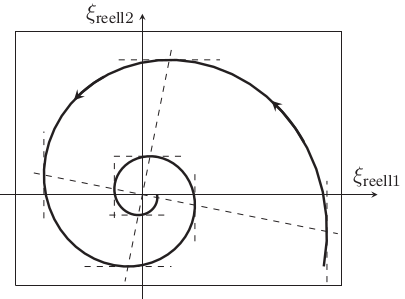
\includegraphics[width=.7\linewidth]{phase-strudel}\\
    \textbf{Wirbelpunkt}\\
    $\lambda_{1/2} = \pm \beta j$: Wirbel in Drehrichtung von $q_r$ ($\xi_{\text{reel}1}$) nach $-q_i$ ($\xi_{\text{reel}2}$)\\
    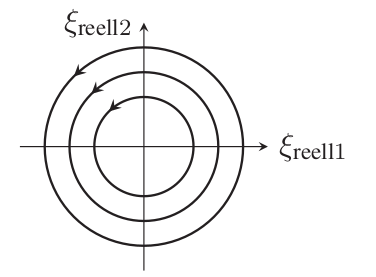
\includegraphics[width=.7\linewidth]{phase-wirbel}\\
    \textbf{Knotenpunkt}\\
    $\lambda_{1,2} < 0, |\lambda_1| < |\lambda_2|$: Trajektorien von Richtung (Eigenvektor) des schnelleren Eigenwerts ($q_2, \xi_2$) schmiegen sich an an Richtung des langsameren Eigenwerts ($q_1, \xi_1$).\\
    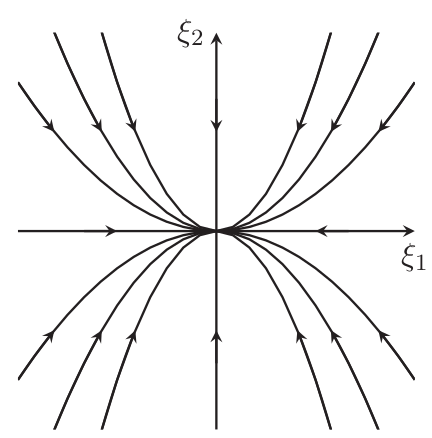
\includegraphics[width=.7\linewidth]{phase-knoten}\\
    \textbf{Sattelpunkt}\\
    $\lambda_1 < 0, \lambda_2 > 0$: Zwei Geraden in Eigenrichtungen, von stabiler Richtung zu GGP, zu instabiler Richtung. Restliche Trajektorien Hyperbeln mit Geraden als Asymptoten.\\
    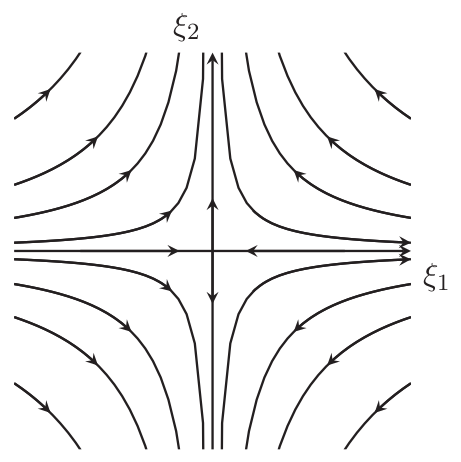
\includegraphics[width=.7\linewidth]{phase-sattel}\\
    %TODO degradierte Phasenportraits? S.60
    \textbf{IV. Einzeichnen von Fixpunkt und Eigenvektoren}\\
    Die Eigenvektoren werden ausgehend vom Fixpunkt eingezeichnet. Bei konjugierten Eigenvektoren zeichnet man den Realteil und den negierten Imaginärteil.\\
    \subsubsection{Isokline}
    Kurve, auf der die Steigung der Trajektorie konstant ist.\\
    $m = \fr {\dot x_1}{\dot x_2}$, falls $m = 0: \dot x_1 = 0$ bzw. $m = \infty: \dot x_2 = 0$
    \subsubsection{Separatrix}
    Kurve, die Gebiete mit verschiedenem Langzeitverhalten trennt.
    \subsection{Lösung der Zustandsgleichungen}
    \subsubsection{Homogener Fall}
    Transformation autonom (konst. Erregung) $\ra$ homogener Fall mit: $\ \v x' = \v x - \v x_\infty$.\\ \\
    $\lambda_1 \neq \lambda_2$: $\v x(t) = \ c_1\e^{\lambda_1t}\v q_1 + c_2\e^{\lambda_2t}\v q_2$\\
    $\lambda_1 = \lambda_2 = \lambda$: $\v x(t) = e^{\lambda t}(\ma 1 + (\ma A -\lambda \ma 1)t) [q_1 q_2]^T$\\
    komplexe Eigenwerte: $c_1 \e^{\alpha t}(\cos{(\beta t)}\v q_{\text{reell}} - \sin{(\beta t)}\v q_{\text{imag}} + c_2\e^{\alpha t}(\sin{(\beta t)}\v q_{\text{reell}} - \cos{(\beta t)}\v q_{\text{imag}})$\\
    \subsubsection{Transformation auf Normalform}
    Gegeben: $\dot{x} = \ma A x$\\
    Normalgleichung: $\dot{\xi} = \Lambda{}\xi$\\
    Eigenwerte $\lambda_1, \lambda_2$ und Eigenvektoren $\v q_1, \v q_2$ berechnen\\
    $\ma Q =  \mat{\v q_1 & \v q_2 }$\\
    $\Lambda = \ma Q^{-1}\ma A\ma Q = \mat{\lambda_1 & 0 \\ 0 & \lambda_2 }, \xi = \ma Q^{-1} x$\\
    $x(t) = \ma Q \xi(t) = \ma Q \exp(\Lambda(t-t_0))\ma Q^{-1} x_0$\\
    \subsubsection{Transformation auf Jordan-Normalform}
    Gegeben: $\lambda = \lambda_1 = \lambda_2, \ma A$ ist keine Diagonalmatrix\\
    $J = \mat{\lambda & 1 \\ 0 & \lambda}, \ma Q' = \mat{\v q_1' & \v q_2'}, \xi'(t) = \ma Q'^{-1}\v x(t)$\\
    Zustandsgleichung in Jordan-Normalform: $\dot \xi '(t) = \ma J \xi '(t)$\\
    Lösung der Zustandsgleichung:\\ $\xi '(t) = \mat{\exp(\lambda(t-t_0))\xi_1'(t_0)+(t-t_0)\exp(\lambda(t-t_0))\xi_2'(t_0) \\ \exp(\lambda(t-t_0))\xi_2'(t_0) }$\\
    Rücktransformation: $\v x(t) = \ma Q'\xi '(t) = \v q_1'\xi_1'(t) + \v q_2'\xi_2'(t)$\\
    \subsubsection{Transformation auf reellwertige Normalform}
    Gegeben: $\lambda_{1/2} = \alpha \pm \beta j, \v q_r, \v q_i$\\
    $\Lambda_\text{reell} =  \mat{\alpha & - \beta \\ \beta & \alpha}$\\
    $Q_\text{reell} = \mat{ q_r & - q_i}$\\
    $x_\text{reell} = \ma Q_\text{reell}^{-1} \e^{\Delta t}\ma Q_\text{reell}$\\
    $\dot{\xi}_\text{reell} (t) = \Lambda_\text{reell}\xi_\text{reell}(t)$\\
    \subsection{Zeitverlauf der Zustandsvariablen}
    Eigenwerte: $\lambda_i = \alpha + j\beta$ mit Dämpfung $\alpha$ und Schwingung $\beta$\\
    \textbf{Stabilität:} stabil, falls $\alpha < 0$, sonst instabil\\
    Schwingung mit Kreisfrequenz $\omega = \beta$\\
    \tablebox{
        \begin{tabular*}{\columnwidth}{l@{\extracolsep\fill}|l} \ctrule
            %TODO evtl. Beispielgraph 73ff.
            Fall & Schwingungsart \\ \cmrule
            $\alpha = 0, \beta \neq 0$ & ungedämpfte Schwingung\\
            $\alpha < 0, \beta \neq 0$ & schwach gedämpfte Schwingung\\
            $\lambda_1 = \lambda_2 < 0, \beta = 0$ \quad & aperiodischer Grenzfall\\
            $\lambda_1 \neq \lambda_2, \beta = 0$ & stark gedämpfte Schwingung\\ \cbrule
        \end{tabular*}
    }
    \subsection{Sprung- und Impulsantwort (analog zu \ref{sec:Sprung- und Impulsantwort})}
    Zustandsgleichung der Form $\dot{\v x}(t) = \ma A\v x(t)+\v bv(t)$.\\
    Ausgangsgleichung der Form $y(t) = \v c^T\v x(t) + dv(t)$.
    \subsubsection{Sprungantwort}

    Sprungantwort $y_\sigma(t) = (d-\v c^T\ma A^{-1}\v b)\sigma (t) + \v c^T\ma A^{-1}\exp{(\ma At)}\v b\sigma(t)$ mit der Sprungfunktion $\sigma(t)$\\ \\
    Für ein stabiles System mit $\lim_{t\rightarrow\infty}\exp{(\ma At)} = \ma 0$ ($\lambda_{\text{real}} < 0$) konvergiert die Sprungantwort wie folgt: $y_{\sigma,\infty} = d + \v c^T\ma A^{-1}\v b$.
    \subsubsection{Impulsantwort}
    $h(t) = \dd t y_\sigma(t)$\\
    $h(t) = d\delta (t) + \v c^T\exp{(\ma At)}\v b\sigma(t)$
    \subsection{Steady-State- und Transientenantwort}
    $\v x(t) = \v x_{\text{trans}}(t) + \v x_{\text{steady}}(t)$
    \subsubsection{Steady-State-Antwort}
    $\v x_{\text{steady}}(t) = \text{Re}\{Y(j\omega)\e^{j\omega t}\}$\\
    $X_{\text{steady}}(t) = H(j\omega) \cdot U_{\text{in}}$
    \subsubsection{Transientenantwort}
    Die Summe der Polstellen von $H(j\omega)$ ist die Transientenantwort.\\
    $\v x_{\text{trans}}(t) = \exp{(\ma At)} \cdot \v x_{\text{trans}}(t)$
    \section{Nichtlineare dynamische Systeme}
    \begin{enumerate}
        \item Alle Fixpunkte bestimmen $\v f(x_\infty) \stackrel{!}{=} \v 0$
        \item Jacobimatrix bestimmen
        \item Fixpunkte in Jacobimatrix einsetzen und Eigenwerte und Eigenvektoren bestimmen
        \item Überprüfen des \textbf{Satzes von Hartmann/Grobmann}: \\Für alle Eigenwerte gilt $Re\{\lambda_i\} \neq 0$
        \item Phasenportrait zeichnen (lokale Phasenportraits stetig verbinden)
    \end{enumerate}
    \subsection{Energiefunktion}
    Eigenschaften: stetig, lokal nicht konstant, auf jeder Trajektorie konstant\\
    Schaltung ist \textbf{konservativ}, falls:\\
    $\dot E = 0 \Leftrightarrow \pd{x_1} E(\v x) \dot x_1 + \pd{x_2} E(\v x) \dot x_2 + \hdots + \pd{x_n} E(\v x) \dot x_n = 0$\\
    Erweiterung des Satzes von Hartmann/Grobmann: Jacobimatrix hat nur imaginäre EW und Schaltung ist konservativ $\Leftrightarrow$ GGP ist Wirbelpunkt\\
    %TODO Schwingkreis S.88
    \subsection{Oszillatoren}
    %TODO Bild von Schaltung und Phasenportrait - S.93
    Schaltung mit periodischem Verlauf der Zustandsgrößen\\
    Voraussetzung: nichtlinear, nur ein Fixpunkt (instabil)\\
    \textbf{Van der Pol-Oszillator:}\\
    \parbox{.5\linewidth}{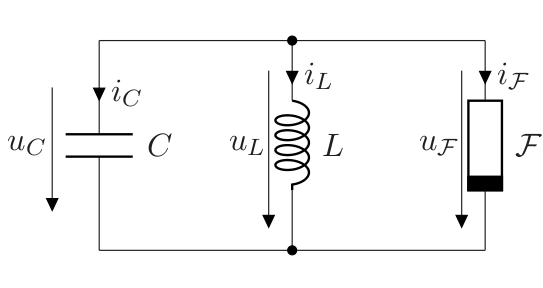
\includegraphics[width=\linewidth]{img/van-der-pol}}
    \parbox{.5\linewidth}{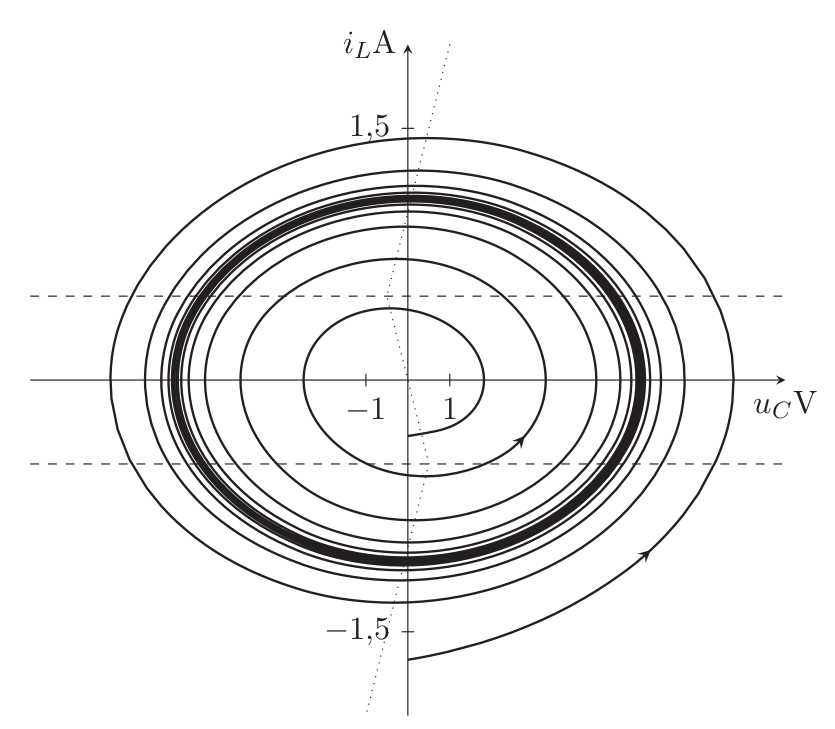
\includegraphics[width=\linewidth]{img/fast-harmonischer-oszillator}}\\
    \textbf{Relaxationsoszillator:}\\
    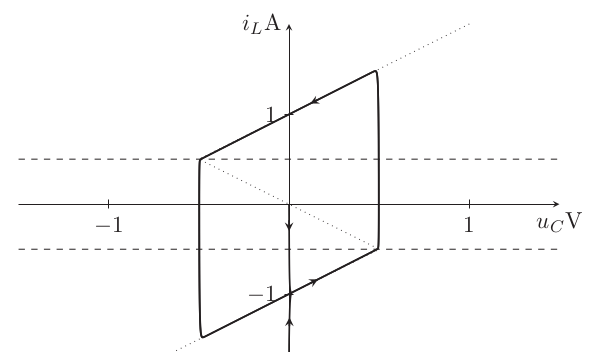
\includegraphics[width=.5\linewidth]{img/relaxationsoszillator}
    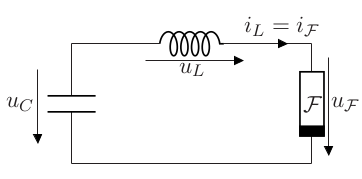
\includegraphics[width=.5\linewidth]{img/relaxationsoszillator-schaltung}
    \section{Dynamische Schaltungen beliebigen Grades}
    %AP und´ Kleinsignalanalyse S.112
    \subsection{Verallgemeinerte Zustandsgleichungen}
    $\dd t \mat{\ma 0 & \ma 0\\\ma 0 & \ma 0\\\ \ma M_1 & \ma N_1}\mat{\v u\\\v i} = - \mat{ \ma B & \ma 0 \\ \ma 0 & \ma A \\ \ma M_0 & \ma N_0}\mat{\v u\\\v i} + \mat{\v 0\\\v 0\\\v e}$\\
    $\ma M_1, \ma N_1$: Elementgleichungen der reaktiven Elemente\\
    $\ma M_0, \ma N_0$: Elementgleichungen aus Tablau\\
    $\ma B$: KVL, $\ma A$: KCL\\
    ($e = 0 \Leftrightarrow$ keine Quellen enthalten)
    \section{Komplexe Wechselstromrechnung}
    \textbf{Vorraussetzung:} lineares, eingeschwungenes System mit sinusförmiger Erregung $x(t) = A_m \cdot \cos(\omega t + \phi)$\\
    \sectionbox{
        \subsection{Komplexe Zeigergrößen}
        \emphbox{
            \begin{tabular}{ll}
                \textbf{Zeitfunktion} & $a(t) = A_m \cdot\cos(\omega t+\phi)$               \\
                \textbf{Zeiger}       & $A = \alpha + i\beta = A_m \cdot e^{i\phi}$         \\
                                      & $=A_m \cdot (\cos \phi+j\sin \phi)$                 \\
                \textbf{Maximum}      & $A_m = |A| = \sqrt{\alpha^2+\beta^2} = \sqrt{AA^*}$ \\
                \textbf{Phase}        & $\phi = \begin{cases}
                        \arctan\frac{\beta}{\alpha}     & \alpha>0 \\
                        \arctan\frac{\beta}{\alpha}+\pi & \alpha<0
                    \end{cases}$
            \end{tabular}
        }

        % ---------------------------------------------------------
        Differentialoperator: $\frac{\diff}{\diff t} = j \omega$\qquad
        $\frac{d}{dt} e^{j(\omega t + \phi)} = j\omega\cdot e^{j(\omega t + \phi)}$\\
        \tablebox{
            \begin{tabular*}{\columnwidth}{l@{\extracolsep\fill}ccc} \ctrule
                & \textbf{Widerstand} & \textbf{Kondensator} & \textbf{Spule}\\ \cmrule
                Impedanz $Z = \frac{U}{I} $ & $R$ & $\frac{1}{j \omega C}$ & $j \omega L$\\
                Admittanz $Y = \frac{I}{U} $ & $G = \frac{1}{R}$ & $j \omega C$ & $\frac{1}{j \omega L}$ \\[0.5em]
                $\underset{\varphi_u - \varphi_i}{\Delta \varphi =}$ & 0 & $-\frac{\pi}{2}$ & $\frac{\pi}{2}$ \\ \cbrule
            \end{tabular*}
        }
    }
    \sectionbox{
        \subsection{Komplexe Leistungsrechnung}
        $U_{\text{eff}} = \frac{1}{\sqrt{2}}U_m$\quad
        $I_{\text{eff}} = \frac{1}{\sqrt{2}}I_m$\\
        \textbf{Momentanleistung}: $p(t) = u(t)i(t)$\\
        \textbf{Energie einer Periode}: $E=\int_0^Tu(t)i(t)dt$\\
        \textbf{Leistungsmittelwert}: $P_w = \frac{1}{T} \int_0^T u(t)i(t)dt$\\
        \textbf{Komplexe Leistung}: $P = \frac{1}{2}UI^* = \frac{1}{2}U_m\cdot e^{j\phi_u}\cdot I_m\cdot e^{-j\phi_i} = U_{\text{eff}}\cdot I_{\text{eff}}\cdot e^{j(\phi_u-\phi_i)}$\\
        \textbf{Scheinleistung}: $S = |P|$\\
        \textbf{Wirkleistung}: $P_w = \text{Re}\{P\}$\\
        \textbf{Blindleistung}: $P_B = \text{Im}\{P\}$
    }
    \section{Analyse dynamischer Systeme im Frequenzbereich}
    \subsection{Laplace-Transformation}
    Für kausale Funktionen mit $f(t) = 0$ für $t < 0$:\\
    $F(p) = \mathcal L\{f(t)\} = \int_0^\infty f(t) \e^{-pt}dt$\\
    Rücktransformation: \\
    $f(t) = \mathcal L^{-1}\{F(p)\} = \fr{1}{2\pi j}\int_{\gamma-j\infty}^{\gamma+j\infty} F(p) \e^{-pt}dt$\\
    \subsubsection{Rechenregeln}
    \begin{itemize}
        \item Linearität: $\mathcal L\{\alpha f(t) + \beta g(t)\} = \alpha F(p) + \beta G(p)$
        \item Differentiationssatz: $\mathcal L\{\dot f(t)\} = pF(p) - f(0)$
        \item Faltung: $\mathcal L\{(a * b)(t)\} = A(p)B(p)$
    \end{itemize}
    \subsubsection{Wichtige Laplace-Transformationen}
    \begin{itemize}
        \item $\mathcal L\{\alpha\e^{\beta t}\} = \fr{\alpha}{p-\beta}$
        \item $\mathcal L\{\e^{\ma At}\} = \fr{1}{p\ma 1 - \ma A}$
    \end{itemize}
    Allgemeine Lösung im Frequenzraum:\\
    $x(p) = \fr{1}{p\ma 1-\ma A}x_0 + \fr{1}{p\ma 1-\ma A}bV(p)$\\
    $x(t) = x(0)\e^{\ma At} + \int_0^t \e^{\ma A(t-t')}v(t')b dt'$
    \subsection{Übertragungsfunktion}
    $H(j\omega ) = \fr{\text{Ausgang}}{\text{Eingang}}$\\
    Nullstellen des Ausgangs werden als $p_{0,i}$ bezeichnet\\
    Nullstellen des Eingangs werden als \textbf{Eigenfrequenzen} $p_{\infty,i}$ bezeichnet\\
    Polstellen $p_{\infty, i}$ von $H(j\omega)$ sind die Eigenwerte der Systemmatrix\\
    \textbf{Bestimmung der Differentialgleichung:}\\
    $H(\j\omega) = \frac{U_A}{U_E} = \frac{a_0 + a_1 \j\omega + a_2 (\j\omega)^2}{e_0 + e_1 \j\omega + e_2 (\j\omega)^2}$\\
    $U_A (e_0 + e_1 \j\omega + e_2 (\j\omega)^2) = U_E  (a_0 + a_1 \j\omega + a_2 (\j\omega)^2)$\\
    $e_0 u_a(t) + e_1 \dot{u}_a(t) + e_2 \ddot{u}_a(t) = a_0 u_e(t) + e_1 \dot{u}_e(t) + e_2 \ddot{u}_e(t)$\\
    3dB-\textbf{Grenzfrequenz:} $\abs{H(j\omega)}^2 = \fr{1}{2}$\\
    \textbf{Stabilität:} Re$\{p_{\infty,i}\} < 0$ \quad $\forall i$\\
    Darstellung einer Schaltung in Abhängigkeit der Frequenz\\
    $H(j\omega) = \abs{H(j\omega)} \exp (j\angle H(j\omega))$\\
    $\phi (\omega) = \angle H(j\omega) = \begin{cases}
            \arctan\frac{\text{Im}\{H(j\omega)\}}{\text{Re}\{H(j\omega)\}}     & $für $\text{Re}\{H(j\omega)\} \geq 0 \\
            \arctan\frac{\text{Im}\{H(j\omega)\}}{\text{Re}\{H(j\omega)\}}+\pi & $für $\text{Re}\{H(j\omega)\} < 0    \\
        \end{cases}$\\
    logarithmierte Darstellung des Betrages: $v(\omega) = 20 \log_{10} \abs{H(j\omega)}$\\
    \subsection{Bodediagramm}
    %TODO Graph, verschiedene Typen (siehe Tut Teutsch)
    \begin{enumerate}
        \item Übertragungsfunktion faktorisieren\\
              $H(jw) = K \cdot \prod_{n=1}^n \left(x_n+\frac{jw}{w_n}\right)^{z_n}$\qquad$z_n \in \mathbb{Z} \ \{0\}$\\
        \item Logarithmierte Beträge der einzelnen Faktoren aufstellen\\
              \quad a) Konstanter Faktor: $y = 20\cdot\log_{10}(K)$dB\\
              \quad b) Falls $x_n = 0$: Gerade durch $(\omega_n, 0$dB$)$\\
              \quad c) Falls $z_n < 0$: Bis $\omega_n$ Funktion gleich 0dB, dann linear um $20 \cdot\log_{10}(x_n)$dB pro Dekade fallend\\
              \quad d) Falls $z_n > 0$: Bis $\omega_n$ Funktion gleich 0dB, dann linear um $20 \cdot\log_{10}(x_n)$dB pro Dekade steigend\\
        \item Phase der Faktoren bestimmen
        \item Logarithmierte Beträge und Phasen aufaddieren
        \item Separates Zeichnen des Betrages $v(\omega)$ und der Phase $\phi(\omega)$ in zwei Diagramme
    \end{enumerate}
    \subsection{Ortskurve}
    \begin{enumerate}
        \item Bestimmung von diversen Werten der Übertragungsfunktion
        \item Eintragen in der komplexen Ebene
        \item Punkte stetig verbinden
    \end{enumerate}
    \parbox{.6\linewidth}{
        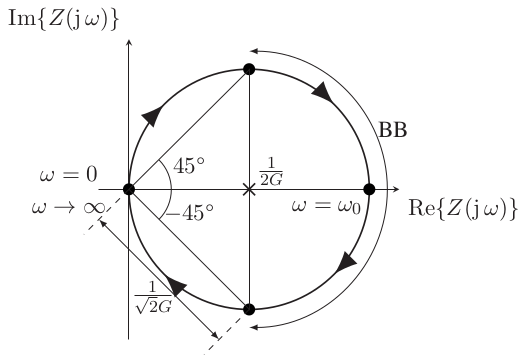
\includegraphics[width=\linewidth]{img/ortskurve-r}}
    \parbox{.4\linewidth}{
        Hier: Widerstandsortskurve eines Parallelschwingkreises. Kann auch Leitwert oder eine andere Übertragungsfunktion sein}
    \subsection{Filtertypen}
    \textbf{Hochpass:} $|H(j0)| = 0, |H(j\omega)| \rightarrow c \text{ für } \omega \rightarrow \infty$\\
    \textbf{Tiefpass:} $|H(j0)| = c, |H(j\omega)| \rightarrow 0 \text{ für } \omega \rightarrow \infty$\\
    \textbf{Bandpass:} $|H(j0)| = 0, |H(j\omega)| \rightarrow 0 \text{ für } \omega \rightarrow \infty, |H(jw_0)| = c$\\
    \textbf{Bandsperre:} $|H(j0)| = c, |H(j\omega)| \rightarrow c \text{ für } \omega \rightarrow \infty, |H(jw_0)| = 0$\\
    \textbf{Allpass:} $|H(j0)| = c$ (Phase kann sich trotzdem abhängig von $\omega$ ändern!)\\
    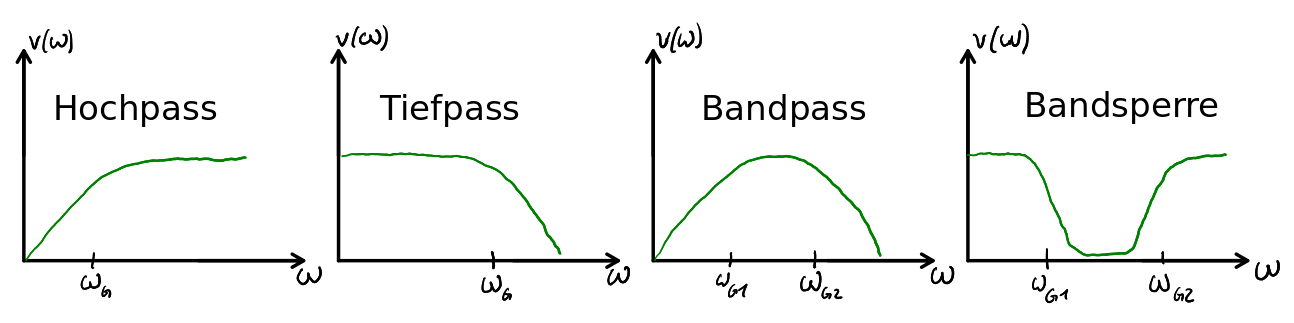
\includegraphics[width=\linewidth]{img/filtertypen}
    \subsection{Schwingkreis}
    Resonanzfrequenz: $\omega_0 = \sqrt{\frac{1}{LC}}$\\
    Gütefaktor: $Q = \frac{\omega_0C}{G} = \frac{1}{\omega_0LG} = \frac{\sqrt{C}}{G\sqrt{L}}$\\
    Eigenfrequenzen: $p_{\infty,1,2} = -\frac{\omega_0}{2Q}\pm \frac{\omega_0}{2Q}\sqrt{1-4Q^2}$
    \section{SPICE}
    \renewcommand{\t}{\texttt}
    \subsection{Bauteile}
    \begin{itemize}
        \item \t{L<Name> <Knoten1> <Knoten2> <Wert>}: Spule zwischen Knoten \t{<Knoten1>} und Knoten \t{<Knoten2>} mit Induktivität \t{<Wert>}
        \item \t{C<Name> <Knoten1> <Knoten2> <Wert>}: Kondensator zwischen Knoten \t{<Knoten1>} und Knoten \t{<Knoten2>} mit Kapazität \t{<Wert>}
        \item \t{R<Name> <Knoten1> <Knoten2> <Wert>}: Widerstand zwischen Knoten \t{<Knoten1>} und Knoten \t{<Knoten2>} mit Widerstandswert \t{<Wert>}
        \item \t{U<Name> <Knoten1> <Knoten2> <Wert>}: Spannungsquelle zwischen Knoten \t{<Knoten1>} und Knoten \t{<Knoten2>} mit Spannung \t{<Wert>} (Spannung positiv bei \t{<Knoten1>})
        \item \t{I<Name> <Knoten1> <Knoten2> <Wert>}: Stromquelle zwischen Knoten \t{<Knoten1>} und Knoten \t{<Knoten2>} mit Stromstärke \t{<Wert>} (Strom in Richtung \t{<Knoten2>})
    \end{itemize}
    \subsection{Parameterbefehle}
    \begin{itemize}
        \item \t{.step param <Param> <Start> <End> <Step>}: Alle Parameter \t{\{<Param>\}} werden vom Startwert \t{<Start>} bis \t{<End>} während der Simulation als Treppenfunktion mit Schrittweite \t{<Step>} eingesetzt.
        \item \t{.step param <Param> list <Wert1> <Wert2> ...}: Simulation wird $n$ mal für jeden Parameterwert durchgeführt.
        \item \t{.step oct param <Param> <Start> <End> <StepsPerOct>}
    \end{itemize}
    \subsection{Analysearten}
    \begin{itemize}
        \item \t{.tran <Endtime>}: Transientenanalyse im Zeitbereich von $t = 0$ bis $t = \text{\t{<Endtime>}}$. Bsp.: \t{.trans 60us}
    \end{itemize}

    \section{Simulink}
    TODO %TODO

\end{multicols*}
\end{document}
